\documentclass[12pt,a4paper]{article}
\usepackage{amsmath,amssymb}
\usepackage{graphicx}
\usepackage{listings}
\usepackage{xcolor}
\usepackage{geometry}
\usepackage{subcaption}
\geometry{margin=2.5cm}

% --- تنظیمات نمایش کدها (Listings) ---
\lstset{
basicstyle=\small\ttfamily,
backgroundcolor=\color{gray!10},
frame=single,
breaklines=true,
postbreak=\mbox{\textcolor{red}{$\hookrightarrow$}\space},
keywordstyle=\color{blue}\bfseries,
commentstyle=\color{green!60!black},
stringstyle=\color{purple},
showstringspaces=false,
columns=fullflexible,
keepspaces=true
}

% --- تنظیمات هایپرلینک ---
\usepackage{hyperref}
\hypersetup{
colorlinks=true,
linkcolor=blue,
urlcolor=cyan
}

% --- تنظیمات زی‌پرشین ---
\usepackage{xepersian}

% تنظیم فونت‌ها
\settextfont{Amiri}
\setlatintextfont{Noto Sans}

\title{\textbf{گزارش جامع راه‌اندازی، پایدارسازی و مصورسازی فریم‌ورک حسگری \lr{Micro-ESPectre} مبتنی بر \lr{ESP32-S3} و پروتکل \lr{MQTT}}}
\author{امیرعلی یزدانی}
\date{\today}

\begin{document}

\maketitle
\tableofcontents
\newpage

\section{مقدمه و هدف پروژه}
هدف از این پروژه، پیاده‌سازی، پایدارسازی و نمایش زنده داده‌های سیستم حسگری حرکت مبتنی بر اطلاعات وضعیت کانال وای‌فای (\lr{WiFi CSI Sensing}) با استفاده از بستر نرم‌افزاری \textbf{\lr{Micro-ESPectre}} بر روی میکروکنترلر \textbf{\lr{ESP32-S3}} است. در این سیستم، تغییرات فاز و دامنه امواج بازتابی ناشی از حرکت افراد پردازش شده و نتایج آن جهت پایش وضعیت محیط منتشر می‌گردد.

\section{آماده‌سازی محیط و نصب سرویس \lr{MQTT}}
برای ایجاد بستر تبادل پیام میان برد \lr{ESP32-S3} و مانیتورینگ، از سرویس کارگزار \lr{Mosquitto} استفاده شد.

\subsection{ساخت فایل پیکربندی سرویس \lr{Mosquitto}}
برای مجاز کردن دسترسی گره‌ها روی پورت استاندارد \lr{1883}، فایل کانفیگ اختصاصی ساخته شد:

\begin{latin}
\begin{lstlisting}[language=bash]
mkdir -p ~/mosquitto_config
cat << 'EOF' > ~/mosquitto_config/mosquitto.conf
listener 1883
allow_anonymous true
EOF
\end{lstlisting}
\end{latin}

\subsection{اجرای کارگزار \lr{Mosquitto} تحت داکر}
کانتینر کارگزار با دستور زیر اجرا و پورت \lr{1883} نگاشت گردید:

\begin{latin}
\begin{lstlisting}[language=bash]
sudo docker run -d 
--name mosquitto 
--restart unless-stopped 
-p 1883:1883 
-v ~/mosquitto_config/mosquitto.conf:/mosquitto/config/mosquitto.conf 
eclipse-mosquitto
\end{lstlisting}
\end{latin}

\subsection{تنظیمات فایروال سیستم}
جهت عبور پکت‌های شبکه از لایه فایروال:

\begin{latin}
\begin{lstlisting}[language=bash]
sudo ufw allow 1883/tcp
\end{lstlisting}
\end{latin}

\section{فلش و دیپلوی فریم‌ورک \lr{Micro-ESPectre}}

\subsection{فلش کردن فریم‌ورک و آماده‌سازی گره}
جهت استقرار مفسر و فریم‌ورک بهینه‌شده \lr{CSI} بر روی برد \lr{ESP32-S3}، حافظه پاک‌سازی و فریم‌ورک اولیه فلش گردید:

\begin{latin}
\begin{lstlisting}[language=bash]
cd ~/Desktop/Amirali/WifiSensing/espectre/espectre/micro-espectre
source venv/bin/activate
./me flash
\end{lstlisting}
\end{latin}

\subsection{تنظیمات فایل پیکربندی}
مشخصات شبکه و اتصال کارگزار در فایل \lr{src/config\_local.py} تنظیم شد:
\begin{latin}
\begin{lstlisting}[language=python]
WIFI_SSID = "Sharif-WiFi"
WIFI_PASSWORD = ""
MQTT_BROKER = "172.27.2.87"
MQTT_PORT = 1883
MQTT_USERNAME = ""
MQTT_PASSWORD = ""
MQTT_TOPIC_PREFIX = "espectre"
\end{lstlisting}
\end{latin}

\subsection{انتقال فایل‌ها و اجرای پروژه}
با استفاده از ابزار خط فرمان پروژه، سورس‌کدها به حافظه گره منتقل و برنامه اجرا شد:

\begin{latin}
\begin{lstlisting}[language=bash]
./me deploy
./me run
\end{lstlisting}
\end{latin}

\section{عیب‌یابی تخصصی حافظه و پایدارسازی جریان \lr{CSI}}

\subsection{شرح خطا و بروز مشکل حافظه (\lr{ENOMEM})}
در زمان اجرای اولیه برنامه با ماژول تولید ترافیک پیش‌فرض (\lr{ICMP Ping})، سیستم با خطای زیر متوقف می‌شد:

\begin{latin}
\begin{lstlisting}
Traffic generator started (ping, 100 pps)
Ping socket error: [Errno 12] ENOMEM
WARNING: Only 0 CSI packets - restarting TG (attempt 2/3)
FATAL: No CSI packets after 3 attempts - cannot operate without traffic
\end{lstlisting}
\end{latin}

\subsection{تحلیل فنی علت بروز خطا}
در پلتفرم \lr{MicroPython}، فراخوانی سوکت‌های خام (\lr{SOCK\_RAW}) برای ارسال بسته‌های پینگ، به ازای هر بسته به بافرهای پیاپی در حافظه \lr{Heap} نیاز دارد. همزمانی ورود فریم‌های حجیم داده \lr{CSI} با این تخصیص‌های مکرر، باعث شکست پیوستگی حافظه شده و سیستم خطای تخصیص حافظه بازمی‌گرداند.
\subsection{راهکار قطعی: سوئیچ به مد \lr{UDP/DNS}}
جهت حذف کامل سربار سوکت‌های خام، مد تولید ترافیک به بسته‌های استاندارد \lr{UDP (DNS Query)} تغییر داده شد. در این حالت به علت ساختار سبک سوکت \lr{UDP}، هیچ‌گونه خطای حافظه‌ای رخ نداد:

\begin{latin}
\begin{lstlisting}[language=python]
#src/traffic.py

def **init**(self, mode=MODE_DNS):
\end{lstlisting}
\end{latin}

\section{مصورسازی داده‌ها در مانیتور تحت وب}

\subsection{باز کردن داشبورد}
جهت پایش بصری وضعیت، فایل رابط کاربری \lr{espectre-monitor.html} موجود در پوشه پروژه، به‌صورت مستقیم با دابل‌کلیک در مرورگر باز شد.

\subsection{تنظیمات اتصال در رابط کاربری}
در کادرهای بالای صفحه، مقادیر زیر وارد و بر روی دکمه \textbf{\lr{CONNECT}} کلیک شد:
\begin{itemize}
\item \textbf{\lr{Broker Address}:} \lr{172.27.2.87}
\item \textbf{\lr{Topic}:} \lr{espectre/node1}
\item \textbf{\lr{Username / Password}:} خالی
\end{itemize}

با برقراری اتصال، نمودار تغییرات دامنه، آستانه حساسیت (\lr{Threshold}) و تشخیص رخداد حرکت به‌صورت بلادرنگ نمایش داده شدند.

\begin{figure}[htbp]
    \centering
    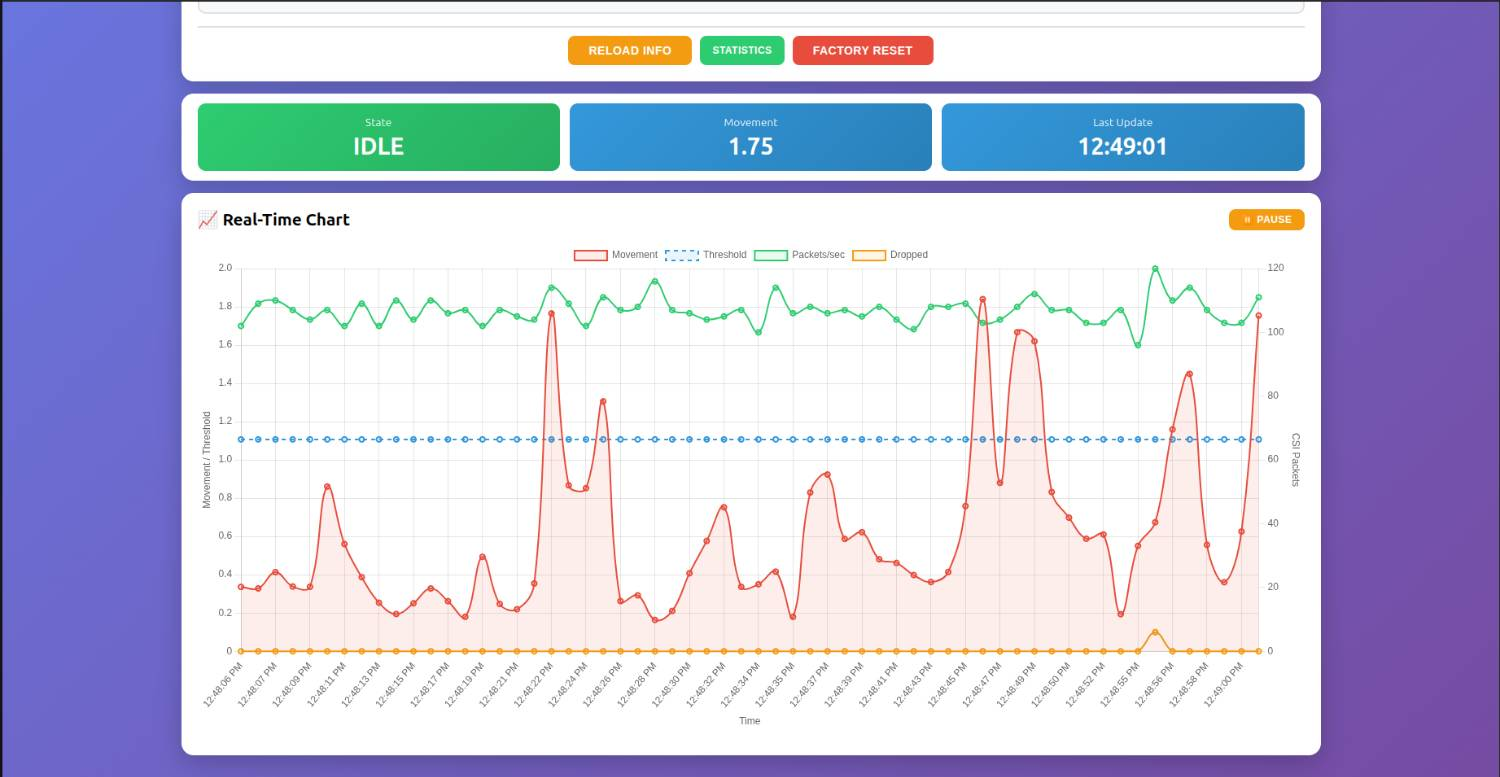
\includegraphics[width=0.85\textwidth]{ImagesPhase5/1.png}
    \caption{نمای داشبورد تحت وب پلتفرم \lr{Micro-ESPectre} پس از برقراری اتصال و مصورسازی بلادرنگ داده‌ها}
    \label{fig:dashboard_espectre}
\end{figure}

\section{مزیت انتخاب پلتفرم \lr{Micro-ESPectre} و چشم‌انداز قابلیت‌های پیشرفته}
هدف اصلی از راه‌اندازی و تثبیت این بستر، بهره‌گیری از ماهیت مفسری و چابک زبان پایتون در پروژه \lr{Micro-ESPectre} در مقایسه با فریم‌ورک‌های سخت و کامپایل‌شونده با \lr{C/C++} نظیر \lr{RuView} است. این پلتفرم امکان ایجاد تغییرات سریع در منطق پردازش سیگنال، تست فیلترهای نویز و نمونه‌سازی الگوریتم‌های هوشمند را بدون اتلاف وقت برای کامپایل‌های طولانی میسر می‌سازد. بر پایه این زیرساخت، پیاده‌سازی اهداف زیر در گام‌های بعدی میسر است:

\subsection{شمارش افراد (\lr{Human Counting / Sensing})}
\begin{itemize}
\item \textbf{امکان‌پذیری:} امکان‌پذیر؛ نیازمند تفکیک تغییرات دامنه امواج ناشی از حضور چندین مانع انسانی مستقل.
\item \textbf{رویکرد پیاده‌سازی:} جمع‌آوری دیتاست برچسب‌خورده با حضور تعداد مشخص افراد در محیط، آموزش مدل رگرسیون پایتونی بر روی ماتریس \lr{CSI}، و فشرده‌سازی مدل نهایی به کمک \lr{TensorFlow Lite Micro} جهت اجرا روی برد.
\end{itemize}

\subsection{مرزبندی و مکان‌یابی فضایی (\lr{Zone Detection / Localization})}
\begin{itemize}
\item \textbf{امکان‌پذیری:} با یک گره منفرد ناممکن است؛ اما با آرایه‌ای از ۲ الی ۳ گره با تکنیک \lr{CSI Fingerprinting} قابل انجام است.
\item \textbf{رویکرد پیاده‌سازی:} ثبت امضای فرکانسی هر بخش از محیط (مانند بخش‌های مختلف اتاق) و دسته‌بندی لحظه‌ای داده‌ها با الگوریتم‌های سبکی نظیر \lr{k-NN} یا \lr{SVM}.
\end{itemize}

\subsection{تشخیص حالت بدنی و ژست (\lr{Posture Detection})}
\begin{itemize}
\item \textbf{امکان‌پذیری:} یک موضوع تحقیقاتی پیشرفته؛ تفکیک وضعیت‌های نشستن، ایستادن و سقوط نیازمند تحلیل بسیار دقیق فاز زیرحامل‌ها است.
\item \textbf{رویکرد پیاده‌سازی:} اعمال شبکه‌های عصبی عمیق (\lr{CNN-LSTM}) بر روی داده‌های زمانی-مکانی استخراج‌شده و اجرای بخش استنتاج مدل بر روی سیستم میزبان.
\end{itemize}

\section{تحلیل معماری خط لوله پردازش سیگنال و الگوریتم تشخیص حرکت (\lr{MVS Pipeline})}
فریم‌ورک \lr{Micro-ESPectre} از الگوریتم \textbf{\lr{Moving Variance Segmentation (MVS)}} جهت استخراج ویژگی و آشکارسازی حضور و حرکت بهره می‌برد. فرآیند تبدیل فریم‌های خام تا تصمیم‌گیری نهایی در چهار گام اصلی صورت می‌پذیرد:

\subsection{استخراج و پاک‌سازی ماتریس دامنه (\lr{Amplitude Extraction})}
بسته‌های دریافتی از درایور وای‌فای حاوی مقادیر مختلط دامنه و فاز ($I$ و $Q$) برای ۶۴ زیرحامل فرکانسی (\lr{Subcarriers}) هستند. در نخستین گام، مقدار دامنه هر زیرحامل از رابطه استاندارد استخراج می‌گردد:
\begin{equation}
\text{Amplitude}_k = \sqrt{I_k^2 + Q_k^2}
\end{equation}
سپس، زیرحامل‌های بدون بار اطلاعاتی (فرکانس مرکزی \lr{DC} و باندهای محافظ \lr{Guard Bands}) جهت کاهش حجم محاسبات و حذف نویز از ماتریس حذف می‌شوند.

\subsection{فیلترینگ میان‌گذر و محاسبه واریانس متحرک (\lr{Moving Variance})}
به دلیل اینکه حرکات بدن انسان نوساناتی در بازه فرکانسی \textbf{۰.۵ الی ۱۰ هرتز} ایجاد می‌کنند، یک فیلتر دیجیتال میان‌گذر روی سیگنال اعمال شده تا تغییرات دمایی محیط و نویزهای فرکانس بالای قطعات فیلتر شوند. 

در ادامه، واریانس لغزان در یک پنجره زمانی متحرک بر روی زیرحامل‌های منتخب محاسبه می‌گردد:
\begin{equation}
\text{Var}(t) = \frac{1}{N} \sum_{i=1}^{N} \left( A_i - \mu \right)^2
\end{equation}
با تجمیع مکانی (\lr{Spatial Aggregation}) مقادیر واریانس تمام زیرحامل‌ها، شاخص نهایی حرکت با نام \textbf{\lr{mvmt}} در بازه مقیاس‌پذیر تولید می‌گردد. در حالت سکون، مقدار شاخص نزدیک به صفر بوده و با شکست مسیرهای چندگانه امواج (\lr{Multipath}) ناشی از تحرک افراد، مقدار آن افزایش می‌یابد.

\subsection{کالیبراسیون اولیه و تعیین آستانه تطبیقی (\lr{Dynamic Thresholding})}
در ابتدای راه‌اندازی (فاز دریافت ۱۰۰۰ پکت نخست)، میانگین و انحراف معیار سطح نویز پایه محیط ($\mu_{\text{noise}}$ و $\sigma_{\text{noise}}$) ثبت می‌شود. مقدار آستانه حساسیت (\textbf{\lr{thr}}) بر اساس رابطه زیر کالیبره می‌گردد:
\begin{equation}
\text{Threshold} = \mu_{\text{noise}} + k \cdot \sigma_{\text{noise}}
\end{equation}

\subsection{ماشین حالت و صدور خروجی (\lr{Decision Engine})}
در حلقه اصلی اجرای پایتون، مقدار شاخص حرکت با آستانه کالیبره‌شده مقایسه شده و وضعیت نهایی به همراه متریک‌ها در قالب بسته \lr{JSON} بر روی تاپیک کارگزار \lr{MQTT} ارسال می‌گردد:
\begin{equation}
\text{State} = 
\begin{cases} 
\textbf{\lr{MOTION}}, & \text{if } \text{mvmt} \ge \text{thr} \\
\textbf{\lr{IDLE}},   & \text{if } \text{mvmt} < \text{thr}
\end{cases}
\end{equation}
جهت پایدارسازی خروجی و جلوگیری از نوسانات سریع بین وضعیت‌ها، یک مکانیزم فیلتر تاخیر زمانی (\lr{Hold Time / Debounce}) پس از قطع حرکت اعمال شده است.

\end{document}